\documentclass[11pt,a4paper]{article}
\usepackage[margin=27mm,headheight=14pt]{geometry}
\usepackage{amsmath,amssymb,amsthm,mathtools,graphicx,booktabs,array}
\usepackage[T1]{fontenc}
\usepackage{lmodern,microtype}
\usepackage{enumitem}
\usepackage{xcolor}
\usepackage[colorlinks=true,linkcolor=blue!45!black,citecolor=blue!45!black,urlcolor=blue!45!black]{hyperref}
\usepackage{fancyhdr}
\pagestyle{fancy}\fancyhf{}
\fancyhead[L]{\small Slope-constrained moment design}
\fancyhead[R]{\small Research draft, 21 September 2026}
\fancyfoot[C]{\thepage}
\setlength{\parskip}{3pt}
\setlength{\emergencystretch}{2em}
\setlist{nosep}
\numberwithin{equation}{section}
\newtheorem{theorem}{Theorem}[section]
\newtheorem{proposition}[theorem]{Proposition}
\newtheorem{lemma}[theorem]{Lemma}
\newtheorem{corollary}[theorem]{Corollary}
\theoremstyle{remark}\newtheorem{remark}[theorem]{Remark}
\DeclareMathOperator{\Lip}{Lip}
\DeclareMathOperator{\sgn}{sgn}
\newcommand{\R}{\mathbb R}
\newcommand{\dd}{\,\mathrm du}
\newcommand{\ds}{\delta_*}
\newcommand{\Ds}{D_*}
\newcommand{\Cs}{C_*}
\newcommand{\rs}{r_*}
\newcommand{\norm}[1]{\lVert#1\rVert}
% Generated from frozen certificate checker outputs by prepare_inputs.py.
\newcommand{\DeltaLower}{9.1787079603827}
\newcommand{\DeltaUpper}{9.1787079608363}
\newcommand{\GammaLower}{1.297542117}
\newcommand{\GammaUpper}{1.297542121}
\newcommand{\CLower}{9.20340371}
\newcommand{\CUpper}{9.20340375}
\newcommand{\KMinus}{9.624\times10^{-33}}
\newcommand{\KPlus}{2.167\times10^{-32}}
\newcommand{\MZero}{2\times10^{-5}}

\title{Amplitude cost of slope-constrained moment design:\\
sharp asymptotics and a validated theta example}
\author{H\"useyin Buldurgan}
\date{21 September 2026\\\small Manuscript core for mathematical review}
\begin{document}
\maketitle
\begin{abstract}
We minimize the amplitude of a bounded multiplier subject to finitely many
exact weighted moments and a separate Lipschitz bound $M$. Under explicit
simple-switch, separation, summability and moment-rank hypotheses, we prove
$\delta(M)=\ds+\Cs M^{-2}+o(M^{-2})$. The coefficient is
$\Cs=\ds^3(3\Ds)^{-1}\sum_k w(z_k)|\rs'(z_k)|$, where $\rs$ is an optimal
weighted $L^1$ residual, $\Ds=\int w|\rs|\dd$, and $z_k$ are its switches.
The upper construction corrects all prescribed moments exactly by moving
finitely many transition centers; the lower bound applies to every
admissible multiplier. For a positive theta kernel at a certified triple
zero, validated arithmetic verifies the hypotheses with infinitely many
switches and encloses $\Cs$ in
$(\CLower,\CUpper)\times10^{-25}$. For every $M\ge\MZero$, the remainder
lies between $-\KMinus/M^3$ and $\KPlus/M^3$. We also explain the relation
to the classical moment duality and the two-parameter Kantorovich--Rubinstein
norm. The numerical statements use analytic bounds and a companion
computation archive; they have not been formally verified or externally refereed.
\end{abstract}
\noindent\textbf{Keywords:} moment problem; amplitude minimization; Lipschitz
constraint; weighted $L^1$ approximation; validated numerics; positive kernels.

\section{Problem and context}\label{sec:intro}
A bounded moment design can have an optimal multiplier that takes just two
values and jumps between them. Requiring a finite slope replaces those
jumps by transitions and increases the minimum amplitude. Our question is
quantitative: how much amplitude must be added when the moments must still
hold exactly? In an oscillatory integral, these moments can pin a zero and
increase its multiplicity while the kernel remains positive.

The setting is the half-line in its given coordinate $u$. For a positive
density $w$, let $d\rho=w(u)\dd$, and let real functions $p_0,\ldots,p_m$
belong to $L^1(\rho)$. Fix $f>0$ and put
\begin{align}
 L_j(h)&=\int_0^\infty p_jh\,d\rho,\qquad
 \mathcal A=\{h:L_j(h)=0\ (j<m),\ L_m(h)=-f\},\label{eq:target}\\
 \ds&=\inf_{h\in\mathcal A\cap L^\infty}\norm h_\infty,\qquad
 \delta(M)=\inf_{\substack{h\in\mathcal A\cap\mathrm{Lip}([0,\infty))\\
                         \Lip(h)\le M}}\norm h_\infty.\label{eq:cost}
\end{align}
Only bounded Lipschitz functions contribute a finite value in the second
infimum. There is no constraint on the total mass of the kernel.
The word \emph{cost} means the relative amplitude $\norm h_\infty$;
it does not mean computation time or a physical resource.

The main result is Theorem~\ref{thm:asymptotic}, with a matching lower and
upper coefficient. Section~\ref{sec:theta} verifies its hypotheses for a
specific theta kernel. Theorem~\ref{thm:remainder} supplies an explicit
bound valid for every sufficiently large slope budget, with a specified
threshold. These results do not characterize the exact finite-$M$
minimizer.

\paragraph{Relation to established work.}
The $L^1$ approximation/$L^\infty$ moment duality is classical; a formulation
of the Markov $L$-moment problem appears in Yuditskii
\cite[Problems 1.2--1.3]{yuditskii}. Perfect-spline extremal problems relate
moments to derivative norms under Chebyshev-system assumptions
\cite[Sections 7--8]{karlin}. The oscillatory functions used here do not
form a global Chebyshev system on the half-line. Amplitude and control-rate
constraints also occur in minimum-time design \cite{albassam}; hence the
idea of imposing a hard slope bound is not new. Bang-bang regularization
uses related information about small switching-function values
\cite{wachsmuth}, but a quadratic penalty parameter cannot be substituted
for our hard bound $M$.

Our auxiliary support functional is exactly the two-parameter
Kantorovich--Rubinstein (KR) norm of Lellmann et al.\ \cite{lellmann}.
Its flat-metric and Wasserstein-type context is developed in
\cite{piccoli,schmitzer}. Section~\ref{sec:dual} records the precise
equivalence, rather than presenting a known norm as a new one. The specific
result studied here is the full coefficient with exact moment preservation,
together with an infinite-switch validated example and a uniform remainder.
The comparison concerns the cited results; it is not a claim that no
equivalent theorem exists elsewhere in the literature.

\section{Duality and normalization}\label{sec:dual}
For $a\in\R^m$, set
\begin{equation}
 r_a=p_m-\sum_{j<m}a_jp_j,\qquad D(a)=\int|r_a|\,d\rho.\label{eq:residual}
\end{equation}
Suppose that $a_*$ satisfies
\begin{equation}
 \int p_j\sgn(r_{a_*})\,d\rho=0\quad(j<m),\qquad
 \Ds=D(a_*)>0.\label{eq:signmoments}
\end{equation}
Write $\rs=r_{a_*}$. Then convexity shows that $a_*$ minimizes $D$.
Moreover
\begin{equation}
 \ds=\frac f\Ds,\qquad h_*=-\ds\sgn\rs.\label{eq:bangbang}
\end{equation}
Indeed $\int p_m\sgn\rs\,d\rho=\Ds$, so $h_*$ is feasible. For every
feasible $h$, $f=|\int\rs h\,d\rho|\le\norm h_\infty\Ds$.
If $\rs\ne0$ almost everywhere, equality forces $h=h_*$ almost everywhere.

For completeness, write $q_j=wp_j$ and define
\begin{align}
 H(A,M;\mu)&=\sup_{\norm g_\infty\le A,\ \Lip(g)\le M}\int g\,d\mu,\label{eq:kr}\\
 V(A,M)&=\sup_{\substack{\norm g_\infty\le A,\ \Lip(g)\le M\\
                         \int q_jg=0\ (j<m)}}\int q_mg.
\end{align}
For $A,M>0$, the exact identities are
\begin{equation}
 \begin{aligned}
 V(A,M)&=\inf_{a\in\R^m}H\left(A,M;(q_m-\textstyle\sum_{j<m}a_jq_j)\dd\right),\\
 \delta(M)&=\inf\{A>0:V(A,M)\ge f\}.
 \end{aligned}\label{eq:krdual}
\end{equation}
To justify minimax, the set $\{|g|\le A,\Lip(g)\le M\}$ is compact and
convex in the topology of uniform convergence on compact intervals by
diagonal Arzel\`a--Ascoli. Its moment maps are continuous: local convergence
handles a compact interval and $A\int_U^\infty|q_j|$ controls the tails
uniformly. Apply Sion's theorem \cite{sion} to the affine Lagrangian.
The infimum over the multipliers $a$ imposes the lower moments exactly.
The second identity follows by scaling a feasible maximizer of $V$ by
$f/V$ whenever $V\ge f$.

Our convention is the \emph{two separate bounds} in \eqref{eq:kr}, with
\begin{equation}
 H(A,M;\mu)=A H(1,M/A;\mu)=M H(A/M,1;\mu).\label{eq:normalization}
\end{equation}
Total variation, if used, is $\int|d\mu|$ without a factor $1/2$.
Zero-extending a measure to the full line gives the same support
functional: a half-line test function extends constantly to the left.
Neither \eqref{eq:krdual} nor our proof assumes that the unrestricted
coefficient $a_*$ remains dual-optimal for finite $M$.

\section{Sharp large-slope asymptotics}\label{sec:general}
Here are the complete local hypotheses used for the asymptotic result.
Assume $m\ge1$, $w>0$, and $w,p_0,\ldots,p_m$ are $C^2$ on the half-line
(one-sided at zero), with $p_j\in L^1(\rho)$. Assume
\eqref{eq:signmoments}. In addition:
\begin{enumerate}[label=(H\arabic*),leftmargin=16mm]
\item $\rs(0)\ne0$, and all positive zeros $z_k$ of $\rs$ are simple.
The zero set is nonempty, finite or countably infinite. The signed set
$\{z_k,-z_k\}$ is uniformly separated by a positive number $d$.
\item For some fixed $b>0$, the intervals $[z_k-b,z_k+b]$ are disjoint
and contained in $(0,\infty)$, and for $0\le j\le m$, $0\le\ell\le2$,
\begin{equation}
 \sum_k\sup_{|u-z_k|\le b}|q_j^{(\ell)}(u)|<\infty.\label{eq:summability}
\end{equation}
\item There are $m$ selected switches such that the matrix
$(p_j(z_k))_{0\le j<m,\ 1\le k\le m}$ is nonsingular, after relabeling.
\end{enumerate}
In particular
\begin{equation}
 0<\Gamma=\sum_k w(z_k)|\rs'(z_k)|<\infty.\label{eq:gamma}
\end{equation}
Finiteness follows from \eqref{eq:summability}, since
$(w\rs)'(z_k)=w(z_k)\rs'(z_k)$.

\begin{theorem}\label{thm:asymptotic}
Under (H1)--(H3) and \eqref{eq:signmoments}, the feasible Lipschitz class is
nonempty for all sufficiently large $M$, and
\begin{equation}
 \boxed{\delta(M)=\ds+\frac{\Cs}{M^2}+o(M^{-2}),\qquad
 \Cs=\frac{\ds^3\Gamma}{3\Ds}=\frac{\ds^4\Gamma}{3f}>0.}\label{eq:main}
\end{equation}
If $\ds<1$, the upper construction has $1+h>0$ for all sufficiently large
$M$. The result is conditional on the stated switch and rank hypotheses.
\end{theorem}

\subsection{Lower bound for all feasible multipliers}
Let $h$ be feasible, $\Lip(h)\le M$, and $\delta=\norm h_\infty$. The exact
duality gap is
\begin{equation}
 (\delta-\ds)\Ds=
 \int_0^\infty |\rs|[\delta+\sgn(\rs)h]\,d\rho.\label{eq:gap}
\end{equation}
The integrand is nonnegative. Fix finitely many switches. At $z_k$, put
$\gamma_k=w(z_k)|\rs'(z_k)|$. In a sufficiently small neighborhood,
$|(w\rs)(z_k\pm v)|\ge(\gamma_k-\varepsilon)v$ and the signs are opposite.
The two bracketed defects $b_\pm$ in \eqref{eq:gap} satisfy
\begin{equation}
 b_++b_-\ge2\delta-2Mv\ge2\ds-2Mv.
\end{equation}
For sufficiently large $M$ integrate over $0\le v\le\ds/M$ to obtain
\begin{equation}
 (\delta-\ds)\Ds\ge
 \sum_{k\in E}(\gamma_k-\varepsilon)
 \int_0^{\ds/M}v(2\ds-2Mv)\,dv
 =\frac{\ds^3}{3M^2}\sum_{k\in E}(\gamma_k-\varepsilon).
\end{equation}
Taking the infimum over $h$, then the lower limit as $M\to\infty$, then
$\varepsilon\downarrow0$, and finally increasing the finite set $E$, proves
$\liminf M^2(\delta(M)-\ds)\ge\Cs$. This order of limits avoids a uniform
Taylor assertion over infinitely many switches.

\subsection{Exact moment correction and the matching upper bound}
Evenly extend the sign profile $s=\sgn\rs$ to the real line. Move only the
selected positive centers to $c_k$, reflect them, and denote the new step
profile by $s_c$. For $a>0$ small set
\begin{equation}
 s_{c,a}(u)=\frac1{2a}\int_{-a}^a s_c(u-v)\,dv,
 \qquad S_j(c,a)=\int_0^\infty q_j(u)s_{c,a}(u)\dd.\label{eq:ramps}
\end{equation}
Transitions are disjoint and avoid zero. Thus $\norm{s_{c,a}}_\infty=1$
and $\Lip(s_{c,a})=1/a$. Negative reflected centers add no transition on
the positive half-line. The jump at a positive switch is
$d_k=2\sgn\rs'(z_k)$.

For an upward unit step at $c$, its change in a moment with density $q$ is
\begin{equation}
 I_q(c,a)=-\frac a2\int_0^1(1-v)[q(c+av)-q(c-av)]\,dv
 =-\frac{a^2}{6}q'(c)+o(a^2).\label{eq:step}
\end{equation}
The same formula defines an even function of signed $a$ at zero. If
$Q_\ell$ bounds $|q^{(\ell)}|$ on the neighborhood, direct differentiation
gives
\begin{equation}
 |I_q|\le a^2Q_1/6,\quad
 |\partial_a I_q|\le |a|Q_1/3,\quad
 |\partial_a^2 I_q|\le Q_1/3+|a|Q_2/12,\quad
 \partial_a^2I_q(c,0)=-q'(c)/3.\label{eq:c2bounds}
\end{equation}
Hypothesis (H2) therefore permits summation and two differentiations of
the local smoothing errors. Only finitely many centers move, so their
center and mixed derivatives are local derivatives. These are sums of
\emph{local differences}, not sums of individual step tails. Consequently
$S_{0:m-1}(c,a)$ has an even $C^2$ extension near $(z,0)$.

At $(z,0)$ its center Jacobian is
\begin{equation}
 J_{jk}=-d_kq_j(z_k),\qquad 0\le j<m,\quad1\le k\le m.\label{eq:centerJ}
\end{equation}
It is nonsingular by (H3). The implicit-function theorem supplies an even
$C^2$ function $c(a)=z+O(a^2)$ with
$S_j(c(a),a)=0$ for every $j<m$.

Let $q_r=w\rs$. Since $q_r(z_k)=0$, moving finitely many centers by
$O(a^2)$ changes its unsmoothed moment by $O(a^4)$. The corresponding
change in the smoothing correction is also $O(a^4)$, by the local $C^2$
bounds. Summing \eqref{eq:step} with the factors $d_k$ yields
\begin{equation}
 S_m(c(a),a)=\int q_rs_{c(a),a}
 =\Ds-\frac{\Gamma a^2}{3}+o(a^2).\label{eq:Sm}
\end{equation}
Define
\begin{equation}
 \alpha(a)=\frac f{S_m(c(a),a)},\qquad h_a=-\alpha(a)s_{c(a),a}.
\end{equation}
All moments in \eqref{eq:target} are exact. Furthermore
\begin{equation}
 \norm{h_a}_\infty=\alpha(a)
 =\ds+\frac{\ds\Gamma}{3\Ds}a^2+o(a^2),\quad
 \Lip(h_a)=\frac{\alpha(a)}a,\quad\alpha'(a)=O(a).
\end{equation}
The map $a\mapsto\alpha(a)/a$ is strictly decreasing for small positive
$a$ and tends to infinity. Thus every sufficiently large $M$ is obtained,
with $a(M)=\ds/M+O(M^{-3})$. Substitution gives the matching upper bound
in \eqref{eq:main}, completing the proof.\hfill$\square$

\begin{figure}[tbp]
\centering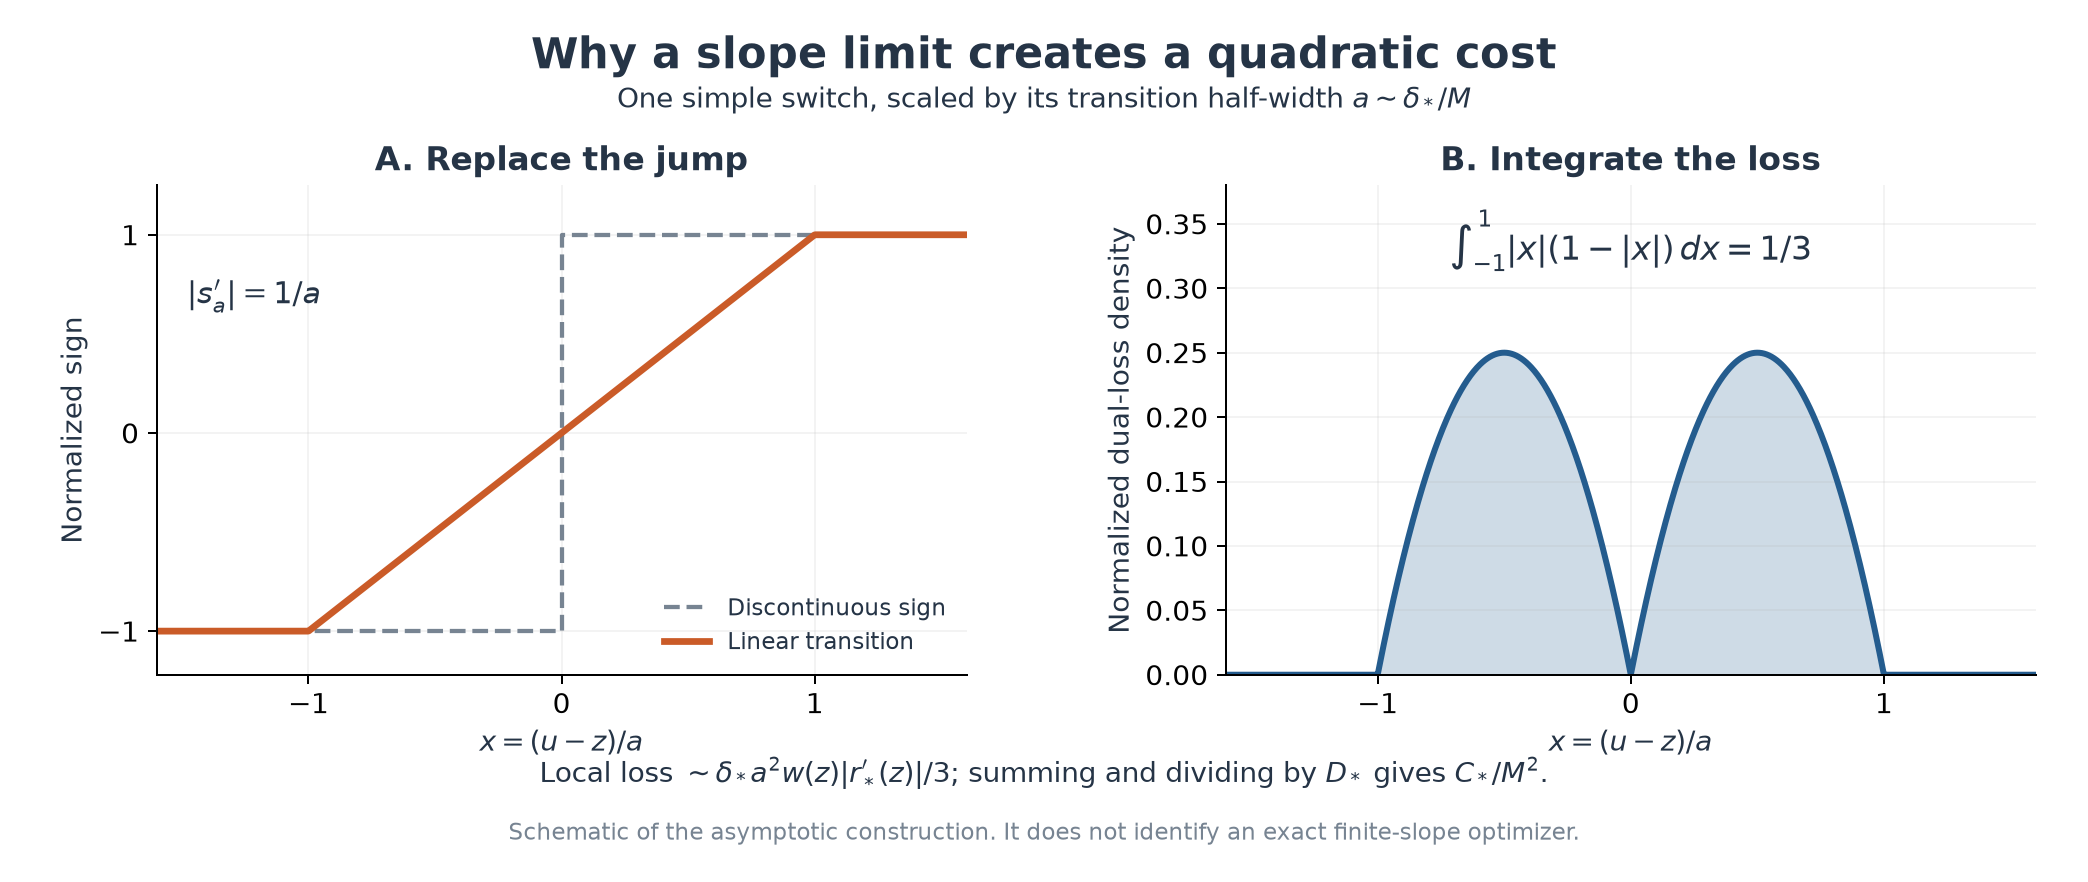
\includegraphics[width=\linewidth]{figures/linear_transition_loss.png}
\caption{The local mechanism behind the coefficient $1/3$. A sign profile
taking values $\pm1$ is replaced locally by a linear transition. The integral of
$|x|(1-|x|)$ on $[-1,1]$ is $1/3$. The figure illustrates the construction;
exact moment correction and the lower bound are supplied by the proof.}
\label{fig:ramp}
\end{figure}

\section{A positive theta kernel at a pinned triple zero}\label{sec:theta}
Consider the fixed-kernel family
\begin{align}
 \Phi(u)&=\sum_{n\ge1}(2\pi^2n^4e^{9u}-3\pi n^2e^{5u})
                  e^{-\pi n^2e^{4u}},\label{eq:kernel}\\
 F_h(t,\lambda,\mu,\nu)&=\int_0^\infty\Phi(u)(1+h(u))
 e^{\lambda u^2+\mu u^4+\nu u^6}\cos(2tu)\dd.\label{eq:family}
\end{align}
Every summand of $\Phi$ is positive for $u\ge0$. Double exponential decay
gives joint analyticity in the four moving coordinates for bounded $h$.
The multiplier $h$ is a single fixed function, independent of those
coordinates.

Let $Q=(\tau,\lambda_Q,\mu_Q,0)$ be the unique solution of
$F_0=(F_0)_t=(F_0)_{tt}=0$ in the exact box of certificate C1
(Appendix~\ref{app:archive}). Its approximate location is
\begin{equation}
 (\tau,\lambda_Q,\mu_Q)\simeq
 (41.40034135868425,-3.645692061604919,
 8.335120498918607).\label{eq:Q}
\end{equation}
These decimals locate $Q$; they do not replace the exact dyadic center and
the certified displacement bound. Set
\begin{equation}
 w=\Phi e^{\lambda_Qu^2+\mu_Qu^4},\qquad
 p_j=(2u)^j\cos(2\tau u+j\pi/2),\qquad f_j=\int p_j\,d\rho.\label{eq:p}
\end{equation}
Here $f_0=f_1=f_2=0$ and $f=f_3>0$. Taking $m=3$ in
\eqref{eq:target} pins $Q$ and makes $\partial_t^jF_h(Q)=0$ for $0\le j\le3$.
It imposes a zero of order \emph{at least} four.

\subsection{The geometric interpretation}
The parameter identities are
\begin{equation}
 (F_h)_\lambda=-\tfrac14(F_h)_{tt},\qquad
 (F_h)_\mu=\tfrac1{16}(F_h)_{t^4},\qquad
 (F_h)_\nu=-\tfrac1{64}(F_h)_{t^6}.\label{eq:heat}
\end{equation}
At the unmodified $Q$, certificate C1 encloses
\begin{equation}
 \begin{gathered}
 3.33563055\times10^{-13}<f_3<3.33563057\times10^{-13},\\
 -9.71679534\times10^{-13}<f_4<-9.71679532\times10^{-13}.
 \end{gathered}
\end{equation}
The two-control determinant is $f_4f_3/64\ne0$. Thus $Q$ is a transverse
triple zero, called a cusp of the equilibrium equation $F_0=0$.
For a local potential with $V_t=F_0$, this is the $A_3$ convention.

Write $g_j=\partial_t^jF_h(Q)$. At the constrained target, direct use of
\eqref{eq:heat} gives
\begin{equation}
 \det\partial_{(\lambda,\mu,\nu)}(g_0,g_1,g_2)
 =\frac{g_4(g_4g_7-g_5g_6)}{4096}.\label{eq:rank}
\end{equation}
A nonzero value ensures both exact order four and rank three of the
unfolding. This is the swallowtail ($A_4$) condition in the potential
convention, not a statement about a fourth-order zero of the original
unmodified transform.

\begin{proposition}\label{prop:smooth}
For this theta example and every $M>0$, $\delta(M)$ is also the infimum
over smooth multipliers with $\Lip(h)\le M$, $\norm h_\infty<1$,
the same four exact moments, and nonzero determinant \eqref{eq:rank}.
This is equality of infima, not attainment in the smooth class.
\end{proposition}
\begin{proof}
The functions $p_0,\ldots,p_N$ are independent on every open interval.
A relation would give $P(u)\cos(2\tau u)+Q(u)\sin(2\tau u)=0$ with
polynomials $P,Q$. Analytic continuation would express $e^{4i\tau z}$
as a rational function unless $P=Q=0$, which is impossible since
$\tau\ne0$. For a nonnegative compactly supported smooth bump $\chi$
positive on an interval, the Gram matrix $B_{ij}=\int\chi p_ip_j\,d\rho$
is positive definite. Hence
\begin{equation}
 R_Nv=\chi\sum_{j=0}^N(B^{-1}v)_jp_j\label{eq:rightinverse}
\end{equation}
is a right inverse of the first $N+1$ moments, bounded in the $C^1$ norm.

Since $\ds<1$ (Table~\ref{tab:cert}), approximate $h_*$ by bounded smooth
compactly supported functions in the weighted moments through order seven.
Use $R_3$ to correct the first four moment errors exactly, and an
arbitrarily small $R_7$ correction in jets $4$--$7$ to avoid the zero set
of the nonzero polynomial in \eqref{eq:rank}. This gives a smooth
feasible anchor $h_0$ with $\norm{h_0}_\infty<1$ and finite slope.
The family $h_\theta=-1+\theta(1+h_0)$, $0<\theta\le1$, remains feasible,
has $1+h_\theta>0$, and has arbitrarily small slope. Its nonzero jets and
determinant scale by $\theta$ and $\theta^3$, respectively.

For any $M>0$ a bounded feasible anchor exists. A minimizing sequence
has a locally uniformly convergent subsequence by Arzel\`a--Ascoli;
integrable tails preserve the moments. Thus a Lipschitz minimizer exists,
and the anchor shows $\delta(M)<1$. Mix it with a smooth anchor of slope
strictly less than $M$. The mixture has a strict slope margin and cost
arbitrarily close to $\delta(M)$. Even extension followed by a nonnegative
even mollifier preserves the amplitude and does not increase the slope.
Moment errors tend to zero. Correct them with $R_3$; then perturb jets
$4$--$7$ with $R_7$ to make \eqref{eq:rank} nonzero. Both $C^1$ corrections
can fit the strict slope and positivity margins. This proves the claim.
\end{proof}

\subsection{Validated hypotheses and the leading coefficient}\label{sec:hypcert}
The weighted $L^1$ objective $D(a)$ is coercive: independence of the first
three $p_j$ gives $\norm{\sum a_jp_j}_{L^1(\rho)}\ge c|a|$.
Every residual is nonzero analytic, so its zeros have measure zero and
$D$ is differentiable, with gradient given by the sign moments.
The following bounds apply to the \emph{exact} $Q$.

\begin{table}[tbp]
\centering\small
\begin{tabular}{p{.40\linewidth}p{.52\linewidth}}
\toprule
Quantity & Certified enclosure or bound\\\midrule
Unrestricted amplitude $\ds$ & $(\DeltaLower,\DeltaUpper)\times10^{-10}$\\
Weighted switch sum $\Gamma$ & $(\GammaLower,\GammaUpper)$\\
Leading coefficient $\Cs$ & $(\CLower,\CUpper)\times10^{-25}$\\
Positive switches in $[0,1]$ & 28 simple roots; 113 complementary sign leaves\\
Tail of $\Gamma$ beyond $u=1$ & $<5.705\times10^{-63}$\\
Signed-switch separation & $>1/200$\\
First three switch moment determinant & positive, approximately $5.30861\times10^{-6}$\\
\bottomrule
\end{tabular}
\caption{Outward decimal bounds from certificates C2--C3. The last
approximation is a locator; exclusion of zero is checked with the exact
interval in C3. No rounded center is treated as an exact optimizer.}
\label{tab:cert}
\end{table}

Certificate C3 starts from an exact dyadic vector $\bar a$, approximately
\begin{equation}
 \bar a\simeq(-0.0001172686588251,
           -0.0646797594922349,
            0.00388087037678106).
\end{equation}
Throughout $\norm{a-\bar a}_\infty\le R=2^{-40}$, it isolates the 28 simple
roots in $[0,1]$ and excludes other roots there by a sign cover. Integrate
the first positive theta summand only over fixed neighborhoods containing
those roots. The Hessian of that part of $D$ is
\begin{equation}
 H(a)=2\sum_{k=1}^{28}
 \frac{w_1(z_k(a))}{|r_a'(z_k(a))|}
 p(z_k(a))p(z_k(a))^T,\quad p=(p_0,p_1,p_2)^T,
\end{equation}
where $w_1$ is that summand times the deformation factor. Positive leading
principal minors certify $H-(1/200)I\succ0$ uniformly. The rest of $D$ is
convex, so $D$ is strongly convex on the cube. Also
$\norm{\nabla D(\bar a)}_1<2.065\times10^{-16}$ and
$R/200-2\norm{\nabla D(\bar a)}_1>4.1345\times10^{-15}$.
Strong convexity makes $D>D(\bar a)$ on the Euclidean sphere of radius $R$,
giving an interior stationary point. Convexity makes it a global
minimizer; local strict convexity rules out any second global minimizer.
Thus the exact $a_*$ is unique and localized in the recorded cube.

For $u\ge1$ the residual is
\begin{equation}
 r_a=A(u)\sin(2\tau u)+B(u)\cos(2\tau u),\quad
 A=8u^3+2a_1u,\quad B=4a_2u^2-a_0.\label{eq:phase}
\end{equation}
The uniform coefficient bounds
$|a_0|<10^{-3}$, $|a_1|<1/10$, $|a_2|<1/200$ imply $A>7u^3$.
With $\vartheta=\arctan(B/A)$,
\begin{equation}
 AB'-BA'=-32a_2u^4+(8a_1a_2+24a_0)u^2+2a_0a_1,
 \quad |\vartheta'|\le(200u^2)^{-1}.
\end{equation}
The phase derivative lies between 81 and 85. Consequently there are
infinitely many simple tail switches, spaced by more than $3/85$.
The finite cover and the transition across $u=1$ complete (H1).

Differentiating the theta series gives, for $\ell=0,1,2$,
\begin{equation}
 |\Phi^{(\ell)}(u)|\le C_\ell
 e^{(9+4\ell)u-\pi e^{4u}},\quad
 \begin{cases}
 C_0=4\pi^2+6\pi,\\
 C_1=60\pi^2+30\pi+16\pi^3,\\
 C_2=660\pi^2+150\pi+448\pi^3+64\pi^4.
 \end{cases}\label{eq:thetaenv}
\end{equation}
For example, the derivative polynomials are generated by
$T(P)=(5-4x)P+4xP'$ from $P_0=-3+2x$.
Their absolute monomial terms have successive-index ratios at most
$256e^{-3\pi}<1/2$; twice the first term bounds each series.
Polynomial factors times this double exponential envelope prove (H2).
The first three switches satisfy (H3). The finite contributions to
$\Gamma$ use 12 theta terms with an explicit series tail; beyond $u=1$
one uses $|r_a'|<900u^3$ and the phase spacing. In particular
\begin{equation}
 \Gamma_{u>1}\le
 \frac{900C_0\exp(9+\mu_+-\pi e^4)}{1-50^{-4}}
 <5.705\times10^{-63},\label{eq:gammatail}
\end{equation}
where $\mu_+$ is the recorded upper bound for $\mu_Q$.
The logarithmic decay rate times $3/85$ exceeds 16 and $e^4>50$;
hence the geometric denominator covers the entire infinite tail.
These checks give Table~\ref{tab:cert} and apply Theorem~\ref{thm:asymptotic}.

\begin{figure}[tbp]
\centering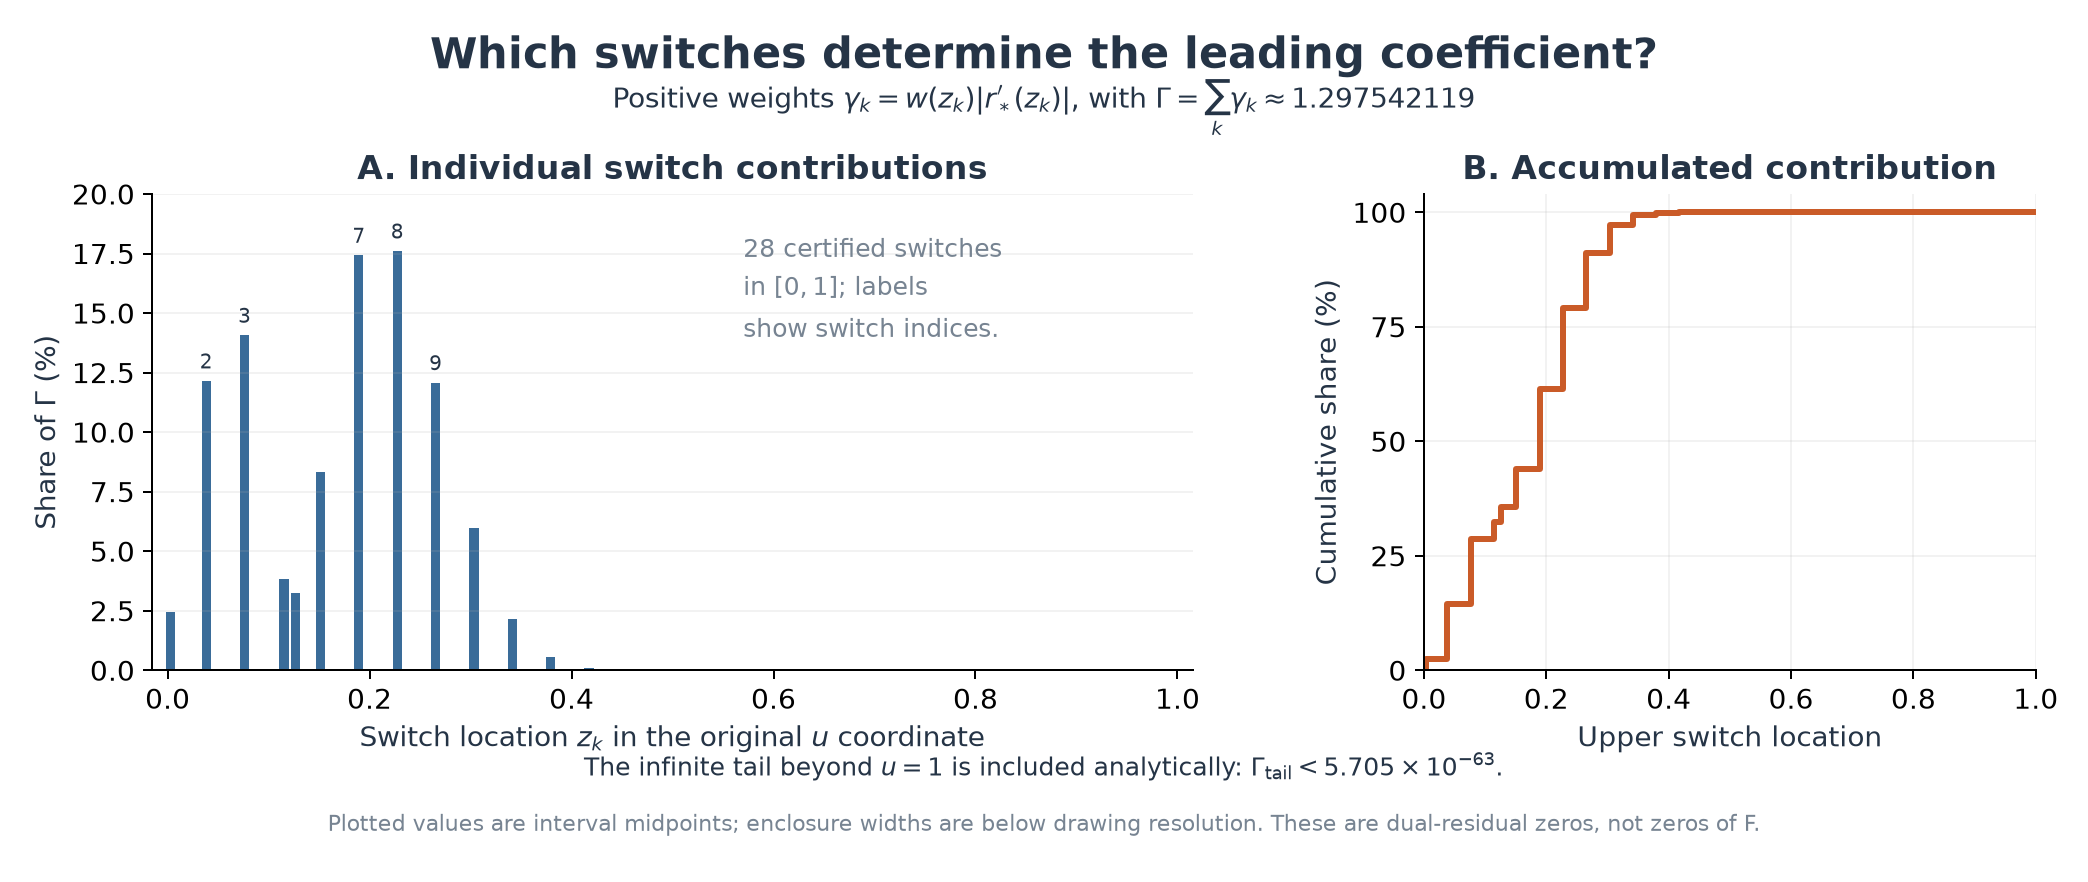
\includegraphics[width=\linewidth]{figures/switch_contributions.png}
\caption{Contributions to $\Gamma$ in the theta example. The plotted values
are interval midpoints, with widths below the drawing resolution; the
infinite tail is included analytically. These switches are zeros of the
optimal dual residual, not zeros of the transform $F_h$.}
\label{fig:switches}
\end{figure}

\section{An explicit uniform remainder}\label{sec:remainder}
\begin{theorem}\label{thm:remainder}
For the exact theta problem in Section~\ref{sec:theta}, for every
$M\ge M_0=\MZero$,
\begin{equation}
 \frac{\Cs}{M^2}-\frac{\KMinus}{M^3}
 <\delta(M)-\ds<
 \frac{\Cs}{M^2}+\frac{\KPlus}{M^3}.\label{eq:remainder}
\end{equation}
In particular
\begin{equation}
 \left|\frac{\delta(M)-\ds}{\Cs/M^2}-1\right|
 <0.001178\frac{M_0}{M}.\label{eq:relerror}
\end{equation}
No sharpness of the order $M^{-3}$ or second asymptotic coefficient is
asserted. The relative error is for the excess above $\ds$.
\end{theorem}

\subsection{Uniform correction over a continuum of transition widths}
Put $a_{\max}=2^{-14}$ and $V=(512,768,384)$. Move only the first three
centers: $c_k=z_k+a^2v_k$, $|v_k|\le V_k$, $0<a\le a_{\max}$.
Let $U_k$ contain the exact root and a radius
$a_{\max}+a_{\max}^2V_k$ for $k\le3$, or $a_{\max}$ otherwise, and define
\begin{equation}
 \begin{gathered}
 Q_{j\ell k}=\sup_{U_k}|q_j^{(\ell)}|,\quad
 R_{\ell k}=\sup_{U_k}|q_r^{(\ell)}|,\\
 B_2=\sum_kR_{2k},\quad A_3=B_2/12,\quad
 A_4=\sum_{k=1}^3(R_{1k}V_k^2+R_{2k}V_k/3).
 \end{gathered}\label{eq:bounds}
\end{equation}
Both $B_2$ and $A_3$ include the infinite tail; $A_4$ includes only the
three moved centers. Certificate C4 supplies
\begin{equation}
 B_2<59.125014562,\qquad A_3<4.927084547,\qquad A_4<132801.204.
\end{equation}
Taylor's theorem in \eqref{eq:step} gives
\begin{equation}
 |I_q(c,a)+a^2q'(c)/6|\le a^3\sup|q''|/24.\label{eq:stepremainder}
\end{equation}
Let $F_j=\frac16\sum_kd_kq_j'(z_k)$ and let $J$ be \eqref{eq:centerJ}.
Then $|S_j(z,a)/a^2+F_j|\le(a/12)\sum_kQ_{j2k}$.
For the exact dyadic preconditioner $B$ recorded in C4, use
\begin{equation}
 T_a(v)=v-BS_{0:2}(z+a^2v,a)/a^2,
 \qquad \norm v_V=\max_k|v_k|/V_k.\label{eq:fixedpoint}
\end{equation}
The exact center derivative is $-d_k$ times the symmetric average of
$q_j$ on $[c_k-a,c_k+a]$. Hence
\begin{equation}
 |\partial_{c_k}S_j-J_{jk}|
 \le\Delta_{jk}:=2a_{\max}^2(V_kQ_{j1k}+Q_{j2k}/6).
\end{equation}
With $E=I-BJ$, define the row bounds
\begin{align}
 \kappa_i&=V_i^{-1}\sum_k
  (|E_{ik}|+\sum_j|B_{ij}|\Delta_{jk})V_k,\\
 \eta_i&=V_i^{-1}\left(|(BF)_i|+
             \frac{a_{\max}}{12}\sum_j|B_{ij}|\sum_kQ_{j2k}\right).
\end{align}
Outward bounds are
\begin{equation}
 \kappa<(0.129747,0.118233,0.071040),\qquad
 \eta<(0.397772,0.406040,0.324017).\label{eq:kappa}
\end{equation}
Thus $T_a$ is a uniform contraction mapping the $V$-box to its interior.
Since $\norm{I-BJ}_V<1$, $BJ$ and therefore $B$ are invertible;
its fixed point solves $S_{0:2}=0$. Also, uniformly in bounded $v$,
\begin{equation}
 S_{0:2}(z+a^2v,a)/a^2=Jv-F+O(a).
\end{equation}
Thus $T_0(v)=(I-BJ)v+BF$ is its continuous extension to $a=0$.
Uniform contraction gives continuous fixed points $v(a)$ for the entire
interval. This is a continuum argument, not a sampling of budgets.

\subsection{Upper and lower error bounds}
Let $L(a)=\Ds-\int q_rs_{c(a),a}$. Positivity of the sign deficit gives
$L\ge0$. Equations \eqref{eq:bounds}--\eqref{eq:stepremainder}, including
the finite center shifts, give
\begin{equation}
 L(a)\le\Gamma a^2/3+A_3a^3+A_4a^4.\label{eq:loss}
\end{equation}
Let $f_-$ be the certified lower bound for $f_3$, and $U_\delta$ the upper
bound for $\ds$. Define
\begin{align}
 D_{\min}&=f_-/U_\delta,\qquad
 E_0=\Gamma_+a_{\max}^2/3+A_3a_{\max}^3+A_4a_{\max}^4,\\
 \overline U&=\frac{U_\delta}{1-E_0/D_{\min}}.\label{eq:Ubar}
\end{align}
Upper bounds are used on the right. C4 checks
$E_0<D_{\min}$, $\overline U<1$, and $\overline U/a_{\max}<M_0$.
For the feasible ramp $h_a=-\alpha(a)s_{c(a),a}$,
$\alpha=f_3/(\Ds-L)$ lies between $\ds$ and $\overline U$.
Continuity, the divergence of $\alpha(a)/a$ at zero, and its value below
$M_0$ at $a_{\max}$ give every $M\ge M_0$ by the intermediate-value
theorem. Monotonicity on this full interval is not required.

Put $e_a=\alpha-\ds$ and choose $a=\alpha/M$. The exact relation is
$\Ds e_a=\alpha L$, so
\begin{equation}
 \Ds e_a\le\frac{\Gamma\alpha^3}{3M^2}
 +\frac{A_3\alpha^4}{M^3}+\frac{A_4\alpha^5}{M^4}.
\end{equation}
Using $\alpha^3-\ds^3\le3\overline U^2e_a$ and absorbing this difference,
\begin{equation}
 e_a-\Cs/M^2\le
 \frac{A_3\overline U^4/M^3+
       (A_4\overline U^5+\Gamma\overline U^2\Cs)/M^4}
      {\Ds-\Gamma\overline U^2/M^2}.\label{eq:absorb}
\end{equation}
The denominator is positive. Exact rational arithmetic on the certified
enclosures gives
\begin{equation}
 \frac{A_3\overline U^4+
 (A_4\overline U^5+\Gamma_+\overline U^2C_+)/M_0}
 {D_{\min}-\Gamma_+\overline U^2/M_0^2}<\KPlus.\label{eq:Kplus}
\end{equation}
Since $\delta(M)\le\alpha$, this proves the upper inequality.

For any admissible $h$, Taylor's theorem gives
$|q_r(z_k\pm v)|\ge P_k(v):=\gamma_kv-R_{2k}v^2/2$.
The true weights and the defects $b_\pm$ in the lower-bound proof are
nonnegative. For $0\le v\le\ds/M$ their paired contribution is at least
\begin{equation}
 \max(0,P_k)(b_++b_-)
 \ge\max(0,P_k)(2\ds-2Mv)\ge P_k(2\ds-2Mv).
\end{equation}
This positive-part step matters when the Taylor lower bound is negative.
Integration gives $\gamma_k\ds^3/(3M^2)-R_{2k}\ds^4/(12M^3)$.
Sum finite sets and pass to the absolutely convergent sums to obtain
\begin{equation}
 \delta(M)-\ds\ge\Cs/M^2-\frac{\ds^5B_2}{12f_3M^3},\qquad
 \frac{U_\delta^5B_2}{12f_-}<\KMinus.\label{eq:Kminus}
\end{equation}
The neighborhoods contain the required intervals for all $M\ge M_0$.
The strict slack in the rounded constants gives \eqref{eq:remainder}.
Dividing by the lower bound on $\Cs$ proves \eqref{eq:relerror}.
\hfill$\square$

At the threshold $M_0$ the total amplitude is enclosed by
\begin{equation}
 \begin{split}
 0.00000000091787309568619750&<\delta(M_0)\\
                          &<0.00000000091787309964331750.
 \end{split}\label{eq:threshold}
\end{equation}
The bound in \eqref{eq:relerror} is below $0.1178\%$ there, for the much
smaller \emph{excess}, not the total amplitude. The theorem applies to the
smooth nondegenerate class as an infimum by Proposition~\ref{prop:smooth}.

\begin{figure}[tbp]
\centering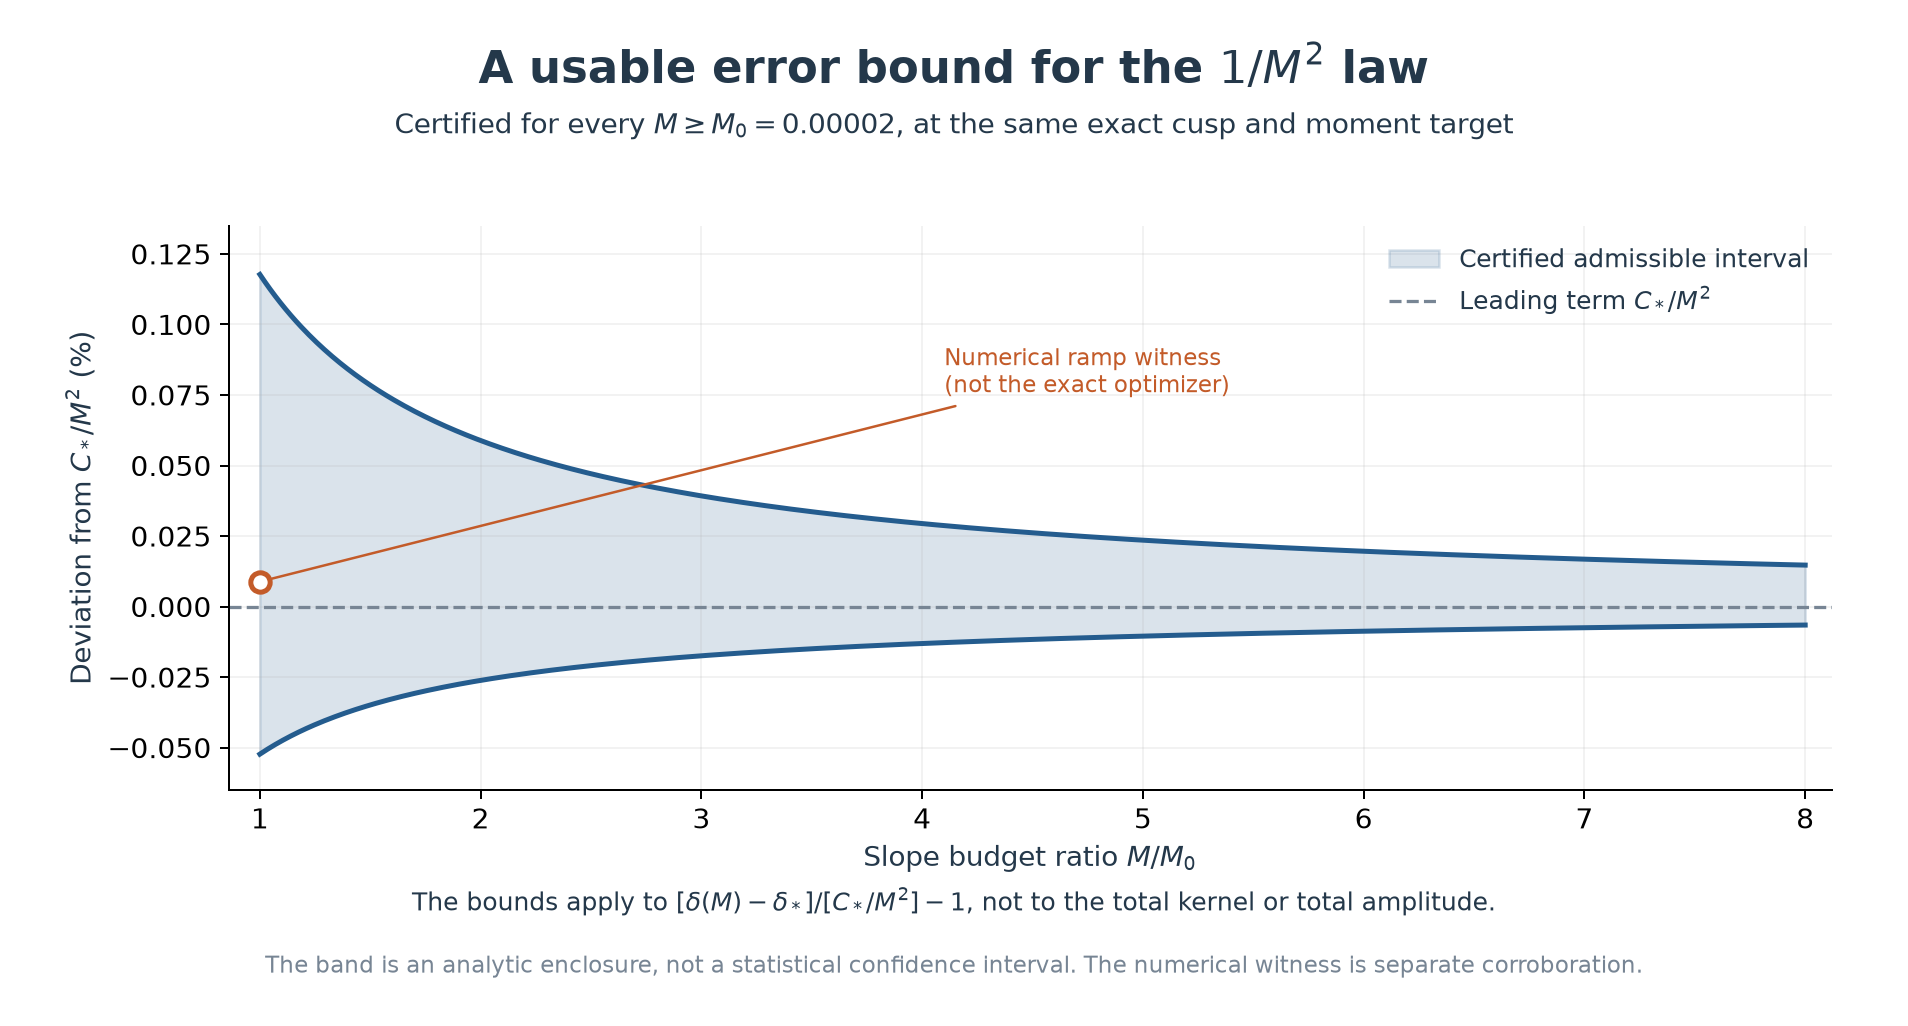
\includegraphics[width=\linewidth]{figures/remainder_envelope.png}
\caption{The enclosure for the deviation from the leading excess
$\Cs/M^2$. The band follows from \eqref{eq:remainder}; it is not a
statistical confidence interval. The hollow point is a separate numerical
ramp witness and does not assert an exact finite-budget optimizer.}
\label{fig:remainder}
\end{figure}

\section{Interpretation and scope}\label{sec:scope}
The baseline amplitude $\ds$ measures the least bounded relative change
that raises the multiplicity at a fixed triple zero. A finite slope adds a
positive cost whose leading coefficient weights every simple switch by the
local density and the slope of the optimal residual. Even though there are
infinitely many switches in this example, their contributions are summable
and the tail is bounded explicitly. The scale and the coefficient depend
on the original coordinate $u$; rescaling that coordinate also rescales the
Lipschitz budget.

The conditional theorem extends beyond the theta density, but it requires
verification of its hypotheses for each new example. It does not cover
multiple residual zeros, accumulating switches, a boundary switch, or a
singular selected moment matrix. The validated application is at one exact
base point $Q$, not a uniform result along the entire cusp curve. It gives
no global count of transform zeros or swallowtails, no result about
undeformed zeta zeros, and no physical model or trained statistical model.
The feasible ramps used for the upper bound are not proved to be the exact
finite-$M$ optimizers, and smooth attainment is not claimed.

\appendix
\section{Certificate interface and reproducibility}\label{app:archive}
The companion research archive contains exact inputs, analytic bounds,
producer programs, separate arithmetic checkers, numerical crosschecks,
and file hashes. Table~\ref{tab:archive} defines the certificate identifiers
used above. Paths are relative to the archive's \texttt{research/} folder.
The full filename in each folder is under \texttt{results/}.

\begin{table}[htbp]
\centering\footnotesize
\begin{tabular}{lll}
\toprule
ID & Folder & Certificate filename\\\midrule
C1 & \texttt{cusp\_verified} & \texttt{quartic\_cusp\_certificate.json}\\
C2 & \texttt{kernel\_norm\_threshold} & \texttt{threshold\_certificate.json}\\
C3 & \texttt{kernel\_slope\_asymptotics} & \texttt{asymptotic\_certificate.json}\\
C4 & \texttt{kernel\_slope\_remainder} & \texttt{remainder\_certificate.json}\\
\bottomrule
\end{tabular}
\caption{Machine-readable companions of the numerical claims. Their
SHA-256 identities and the claim-to-source map are recorded in the
manuscript package. The archive is presently a local research artifact;
a public version and persistent identifier remain to be assigned.}
\label{tab:archive}
\end{table}

\paragraph{Arithmetic representation and the base point.}
A recorded ball has midpoint $m2^e$ and radius $r2^s$, with exact integers.
The enclosing set is $[m2^e-r2^s,m2^e+r2^s]$; printed decimal summaries are
not inputs. C1 applies a fixed-preconditioner contraction to
$G=(F_0,(F_0)_t,(F_0)_{tt})$ on a cube of radius approximately $10^{-24}$.
With a uniform Hessian bound $M_2$, it verifies
$q=\norm{I-YDG(x_0)}+\norm Y M_2R<5.408\times10^{-13}$ and
$\eta+qR<R$, where $\eta=\norm{YG(x_0)}$. Nonsingularity of $Y$ and
Banach's theorem give the unique zero and
$\norm{Q-x_0}_\infty\le\eta/(1-q)<9.099\times10^{-88}$.
Derivative uncertainty is propagated from the exact center to that root.

The finite theta sum is integrated on $[0,U]$ with validated complex
quadrature using Arb \cite{johansson,johanssonintegration}; separate bounds
cover the omitted theta terms and $u>U$. For $C_0$ in
\eqref{eq:thetaenv} and $P^+(u)=\lambda_+u^2+\mu_+u^4+\nu_+u^6$, where
each coefficient is the maximum of zero and its upper parameter-box bound,
one may use
\begin{equation}
 \begin{gathered}
 \int_U^\infty |\partial_t^n(\Phi e^P\cos(2tu))|\dd
 \le\frac{C_0(2U)^n}{c_n}e^{9U+P^+(U)-\pi e^{4U}},\\
 c_n=4\pi e^{4U}-9-n/U-(P^+)'(U)>0.
 \end{gathered}
\end{equation}
The choice of $U$ also makes each positive polynomial derivative term
times $e^{-4u}$ nonincreasing, so the bound holds on the entire tail.
C1 uses $U=2$, 16 theta terms and 110 decimal working precision, with a
separate higher-precision check. C2 obtains a lower amplitude bound from
an upper bound for $D$, and an upper amplitude bound from an exactly
moment-corrected feasible design. Thus the two certificate directions
are not interchanged.

\paragraph{Remainder derivative tails.}
C4 uses \eqref{eq:thetaenv} and $|P'|\le44(1+u)^3$,
$|P''|\le116(1+u)^2$. Let
\begin{align}
 W_0&=C_0,& W_1&=C_1+44C_0,& W_2&=C_2+88C_1+2052C_0,\\
 T_{j0}&=2^jW_0,& T_{j1}&=2^j[W_1+(j+84)W_0].
\end{align}
For $j\le3$ set
$T_{j2}=2^j[W_2+2(j+84)W_1+(j(j-1)+168j+7056)W_0]$.
Then, for $0\le\ell\le2$,
\begin{equation}
 |q_j^{(\ell)}(u)|\le T_{j\ell}(1+u)^9
 \exp(17u+\mu_+u^4-\pi e^{4u}).
\end{equation}
For $u_0=1-a_{\max}$ the logarithmic decay rate of this envelope is at
least $c=4\pi e^{4u_0}-4\mu_+u_0^3-17-9/(1+u_0)$ throughout $u\ge u_0$.
Since $c(3/85)>16$, the sum of neighborhood suprema is bounded by the
envelope at $u_0$ divided by $1-50^{-4}$. Combining these bounds with the
coefficient bounds gives the $q_r$ tails. Finite interval evaluations
and these infinite-tail bounds, rather than samples of derivatives,
supply the constants in \eqref{eq:bounds}.

\paragraph{Checks and trust boundary.}
The recorded runtime is Python 3.12.14, python-flint 0.9.0 and FLINT 3.6.0.
Separate rational checkers reconstruct the containment, sign, contraction
and remainder inequalities from dyadic balls. Independent mpmath runs
corroborate selected roots, integrals and coefficients, but do not replace
interval enclosures. File hashes establish provenance, not mathematical
validity. The analytic proofs and interval computations depend on the
correctness of the stated bounds, producer code and arithmetic libraries;
there is no proof-assistant verification or independent referee report.
Reproduction commands and the complete source map are in the companion
\texttt{manuscript\_core/README.md} and \texttt{CLAIM\_SOURCE\_MAP.md}.

\begin{thebibliography}{99}\small\raggedright
\bibitem{yuditskii} P. Yuditskii, On the $L^1$ extremal problem for entire
functions, \emph{J. Approx. Theory} 179 (2014), 63--93.
\href{https://doi.org/10.1016/j.jat.2013.11.011}{doi:10.1016/j.jat.2013.11.011}.
\bibitem{karlin} S. Karlin, Interpolation properties of generalized perfect
splines and the solutions of certain extremal problems. I,
\emph{Trans. Amer. Math. Soc.} 206 (1975), 25--66.
\href{https://doi.org/10.1090/S0002-9947-1975-0367512-0}{doi:10.1090/S0002-9947-1975-0367512-0}.
\bibitem{albassam} B. A. Albassam, Optimal near-minimum-time control design
for flexible structures, \emph{J. Guidance Control Dynam.} 25 (2002), 618--625.
\href{https://doi.org/10.2514/2.4945}{doi:10.2514/2.4945}.
\bibitem{wachsmuth} D. Wachsmuth, Adaptive regularization and discretization
of bang-bang optimal control problems, \emph{Electron. Trans. Numer. Anal.}
40 (2013), 249--267.
\href{https://etna.ricam.oeaw.ac.at/vol.40.2013/pp249-267.dir/pp249-267.pdf}{Journal full text}.
\bibitem{lellmann} J. Lellmann, D. A. Lorenz, C. Sch\"onlieb and T. Valkonen,
Imaging with Kantorovich--Rubinstein discrepancy,
\emph{SIAM J. Imaging Sci.} 7 (2014), 2833--2859.
\href{https://doi.org/10.1137/140975528}{doi:10.1137/140975528}.
\bibitem{piccoli} B. Piccoli and F. Rossi, On properties of the generalized
Wasserstein distance, \emph{Arch. Ration. Mech. Anal.} 222 (2016), 1339--1365.
\href{https://doi.org/10.1007/s00205-016-1026-7}{doi:10.1007/s00205-016-1026-7}.
\bibitem{schmitzer} B. Schmitzer and B. Wirth, A framework for Wasserstein-1-type
metrics, \emph{J. Convex Anal.} 26 (2019), 353--396.
\href{https://journalofconvexanalysis.com/articles/jca26020/}{Journal article page}.
\bibitem{sion} M. Sion, On general minimax theorems,
\emph{Pacific J. Math.} 8 (1958), 171--176.
\href{https://doi.org/10.2140/pjm.1958.8.171}{doi:10.2140/pjm.1958.8.171}.
\bibitem{johansson} F. Johansson, Arb: efficient arbitrary-precision
midpoint-radius interval arithmetic, \emph{IEEE Trans. Comput.}
66 (2017), 1281--1292.
\href{https://doi.org/10.1109/TC.2017.2690633}{doi:10.1109/TC.2017.2690633}.
\bibitem{johanssonintegration} F. Johansson, Numerical integration in
arbitrary-precision ball arithmetic, in \emph{Mathematical Software---ICMS
2018}, Lecture Notes in Computer Science (2018), 255--263.
\href{https://arxiv.org/abs/1802.07942}{arXiv:1802.07942}.
\end{thebibliography}
\end{document}
